%DEBUT EnTete
\documentclass[10pt,a4paper]{article}
\usepackage[T1]{fontenc}
\usepackage{amsmath}
\usepackage{amsfonts}
\usepackage{amssymb}
\usepackage{graphicx}
\usepackage{calc}
\usepackage{pgf,tikz}
%https://stackoverflow.com/questions/67845020/how-to-avoid-latex-error-environment-axis-undefined-when-using-include-tikz : 
\usepackage{pgfplots}
% https://tex.stackexchange.com/questions/81899/what-does-running-in-backwards-compatibility-mode-mean-and-what-should-i-fix-t
\pgfplotsset{compat=1.17}
\usepackage{pstricks-add}
\usetikzlibrary{arrows}
\usepackage{mathrsfs}
\usepackage{ifthen}
\usepackage{pdfpages}
\usepackage[left=2cm,right=2cm,top=2cm,bottom=2cm]{geometry}
\usepackage{datatool}
\everymath{\displaystyle}
\usepackage{fancyhdr} 
\usepackage{hyperref}
\usepackage{calculator}
%\usepackage{sagetex}
%FIN EnTete
%DEBUT MesCommandes

\setlength{\parindent}{0em}



% *********************************************************************
% MODIFIER LA LIGNE SELON LE MODE VOULU : **********************
\newcommand{\EnonceCorrection}{C}	% E = mode énoncé   C = mode correction 
% **********************************************************************



%%%%%%%%%%%%% MetaDonnees.tex %%%%%%%%%%%%%%%%%%%%%
\newcommand{\AfficheMetaAuteur}{
% Pour imprimer les métadonnées (à effacer) : 
{\bf Auteur : \AuteurEx    \hfill Nom de l'exercice : \varnom  \hfill  Version :   \VersionEx }

{\bf Date de création : \DateCreationEx \hfill Date de modification : \DateModificationEx }

{\bf Source de l'exercice : \SourceEx }

{\bf Description : \DescriptionEx}

\hrulefill

}
%%%%%%%%%%%%% TitreDuTexte %%%%%%%%%%%%%%%%%%%%%
% #1 :  niveau                   #2 : Titre
\newcommand{\TitreDuTexte}{
{\bf \varnom \large   \hfill \NiveauEx Mathématiques \hfill   $ e^{i\pi}+1=0$ }

\bigskip
\centerline{\bf \large \NomEx}
\bigskip
}

%%%%% Quelques commandes personnalisées %%%%%%%%%%%%%%%%%%
\newcommand{\euro}{\eurologo{}} 
\newcommand{\e}{\mbox{e}}
\newcommand{\R}{\mathbb{R}}
\newcommand{\N}{\mathbb{N}}
\newcommand{\D}{\mathbb{D}}
\newcommand{\Z}{\mathbb{Z}}
\newcommand{\Q}{\mathbb{Q}}
%\newcommand{\C}{\mathbb{C}}
\renewcommand{\mathbf}{}
\renewcommand{\vec}[1]{\overrightarrow{#1}}

%============================================================
% POUR L'ENONCE : Le paramètre est l'énoncé \enonce{Ceci est l'énoncé}
\newcommand{\enonce}[1]{
% \EnonceCorrection = E (énoncé seulement) ou C (énoncé et correction)
\ifthenelse{\equal{\EnonceCorrection}{E}}{#1}{ {\bf \it #1}}{} }

% POUR LA CORRECTION : Le paramètre est la solution \correction{Ceci est la correction}
\newcommand{\correction}[1]{
% \EnonceCorrection = E (énoncé seulement) ou C (énoncé et correction)
\ifthenelse{\equal{\EnonceCorrection}{C}}{ \ \ \newline 
 {\bf SOLUTION : } #1}{}
}

% VARIABLE points par exercices 
%\newcounter{pointsexercice}
% Cette variable se remets à 0 à chaque début d'exercice par la commande : \setcounter{pointexercice}{0}
%\COPY{0}{\pointexercice}

% VARIABLE qui contient le total des points 
\newcounter{pointssujetTOTAL}
\setcounter{pointssujetTOTAL}{0}
\COPY{0}{\pointssujetTOTAL}

% VARIABLE qui contient le numéro de l'exercice : 
\newcounter{numeroexercice}

\newcommand{\Affichepointsexercice}{
% \EnonceCorrection = E (énoncé seulement) ou C (énoncé et correction)
\ifthenelse{\equal{\EnonceCorrection}{C}}{  \ \ \hfill {\bf  Cet exercice comporte  $\pointexercice$  points }}{}

}

\newcommand{\AffichepointssujetTOTAL}{
% \EnonceCorrection = E (énoncé seulement) ou C (énoncé et correction)
\ifthenelse{\equal{\EnonceCorrection}{E}}{ \ \ \newline  {\bf Le sujet compte un total de $\pointssujetTOTAL$ \ points.} }{}
}

% \newcommand{\points}[1]{\setcounter{pointsexercice}{\thepointsexercice + #1} {\bf [#1 point(s)]}} 
\newcommand{\points}[1]{\ADD{#1}{\pointexercice}{\pointexercice} \ADD{#1}{\pointssujetTOTAL}{\pointssujetTOTAL}  {\bf [#1 point(s)]}}

\newcommand{\poids}[1]{ {\bf [poids = #1 \%]}}

\newcommand{\EXERCICE}{
% On ajoute 1 au numéro de l'exercice :
\setcounter{numeroexercice}{\thenumeroexercice + 1}
% On remet à zéro les points de l'exercice 
\COPY{0}{\pointexercice}

\bigskip
{\bf EXERCICE \thenumeroexercice \ (Tous les résultats doivent être justifiés)} 

}
% Cette commande insère une nouvelle page en mode ENONCE 
\newcommand{\NouvellePageModeEnonce}{
% \EnonceCorrection = E (énoncé seulement) ou C (énoncé et correction)
\ifthenelse{\equal{\EnonceCorrection}{E}}{{\ } \newpage }{} }

% Cette commande insère une nouvelle page en mode CORRECTION 
\newcommand{\NouvellePageModeCorrection}{
% \EnonceCorrection = E (énoncé seulement) ou C (énoncé et correction)
\ifthenelse{\equal{\EnonceCorrection}{C}}{{\ }  \newpage }{} }


% Cette commande seulement mode ENONCE 
\newcommand{\SeulementModeEnonce}[1]{
% \EnonceCorrection = E (énoncé seulement) ou C (énoncé et correction)
\ifthenelse{\equal{\EnonceCorrection}{E}}{ #1 }{} }

% Cette commande seulement en mode CORRECTION 
\newcommand{\SeulementModeCorrection}[1]{
% \EnonceCorrection = E (énoncé seulement) ou C (énoncé et correction)
\ifthenelse{\equal{\EnonceCorrection}{C}}{ #1 }{} }

% Commande balise pour définir une variable : \var{p}{10} affichera juste 10, mais 
% le programme reconnaitra la variable p 
\newcommand{\var}[2]{\fbox{$#2$}_{\fbox{\mbox{\bf #1}}}}


%FIN MesCommandes
%DEBUT MetaAuteur
\newcommand{\AuteurEx}{} 
\newcommand{\VersionEx}{} 
\newcommand{\DateCreationEx}{} 
\newcommand{\DateModificationEx}{} 
\newcommand{\SourceEx}{} 
\newcommand{\NotionsEx}{} 
\newcommand{\NiveauEx}{} 
\newcommand{\NomEx}{}
%FIN MetaAuteur

\begin{document}
\EXERCICE
\SeulementModeEnonce{\poids{100} }
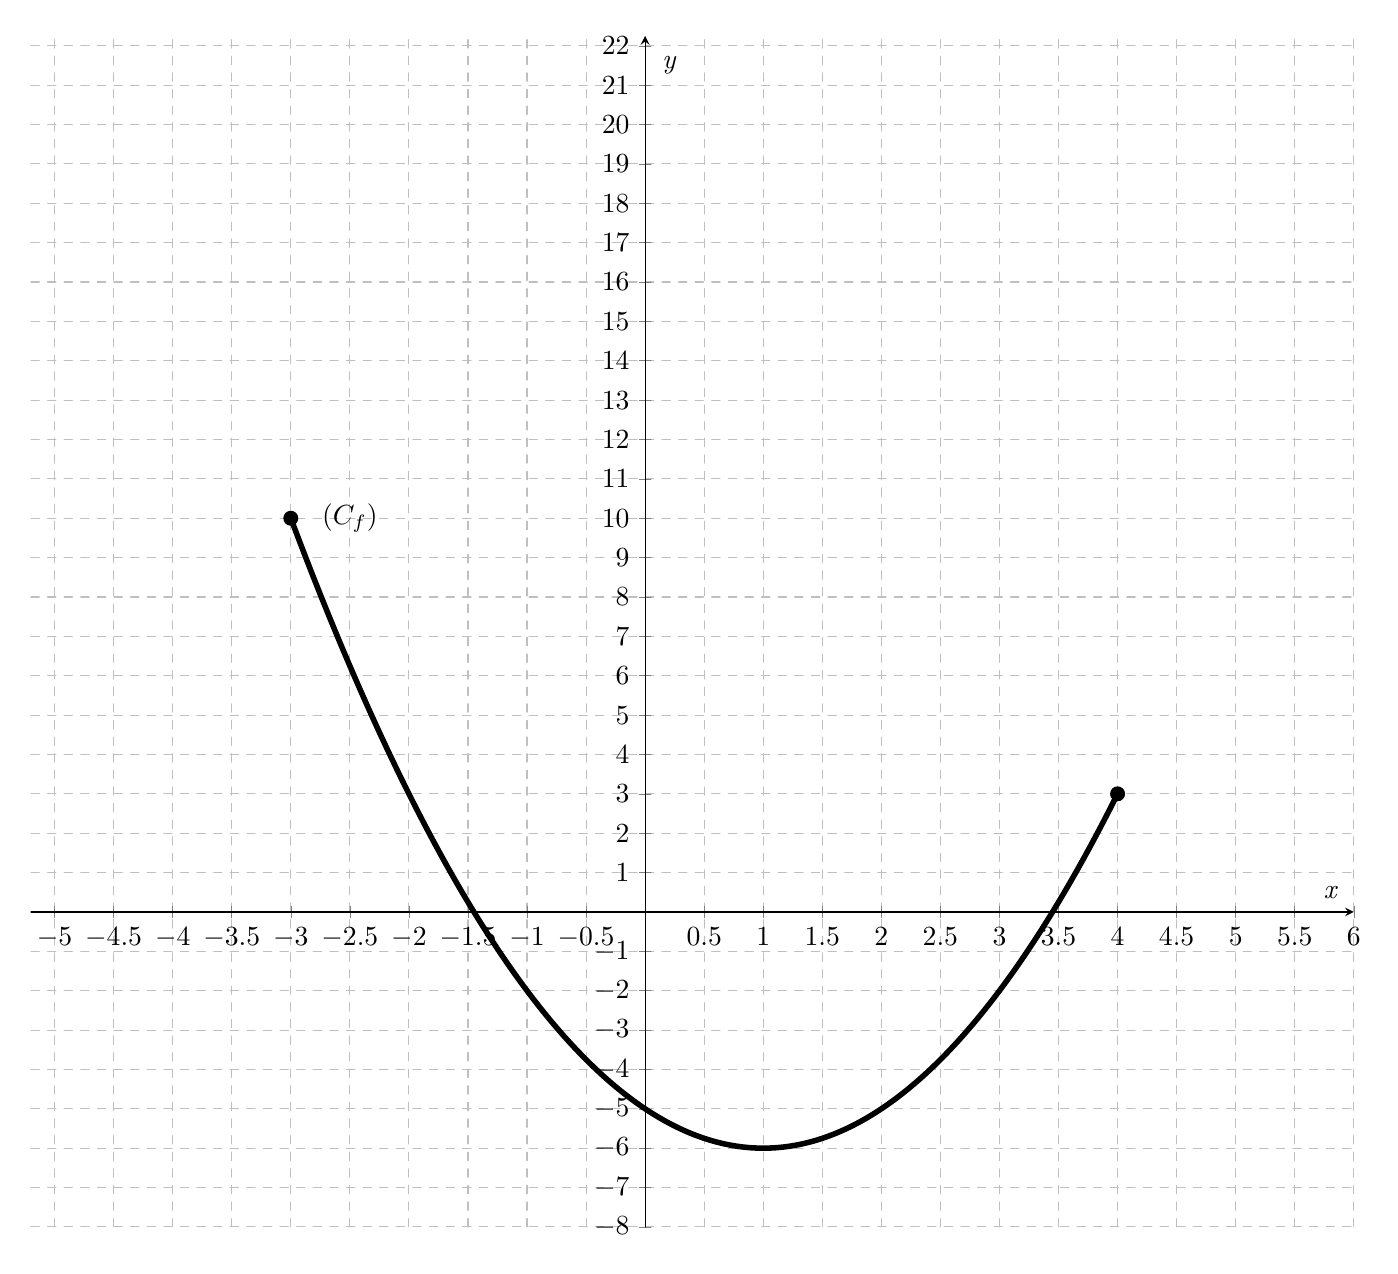
\begin{tikzpicture}[line cap=round,line join=round,>=triangle 45,x=1.0cm,y=1.0cm]
\begin{axis}[
x=1.5cm,y=0.5cm,
axis lines=middle,
grid style=dashed,
ymajorgrids=true,
xmajorgrids=true,
xmin=-5.2,
xmax=6,
ymin=-8.0,
ymax=22.25,
xtick={-5.0,-4.5,...,6},
ytick={-8.0,-7.0,...,22.0},]
\clip(-5.17031,-8.06760180995476) rectangle (8.9,22.2);
%\draw[line width=2.pt,smooth,samples=100,domain=\var{xA}{-3}:\var{xB}{4.}] plot(\x,{\var{ftikz}{(\x)^(2.0)-2*(\x)-5}});
\draw[line width=2.pt,smooth,samples=100,domain=-3.0:4.0] plot(\x,{(\x)^(2.0)-2*(\x)-5});
\begin{scriptsize}
\draw[color=black] (-2.5,10.0) node {$(C_f)$};
\draw[color=black] (5.8,0.5) node {{\bf\it x}};
\draw[color=black] (0.2,21.5) node {{\bf\it y}};
%\draw [fill=black] (\var{xA}{-3},10.) circle (2.5pt);
\draw [fill=black] (-3.,10.) circle (2.5pt);
%\draw [fill=black] (\var{xB}{4.},3.) circle (2.5pt);
\draw [fill=black] (4.0,3.) circle (2.5pt);
\end{scriptsize}
\end{axis}
\end{tikzpicture}

On considère $(C_f)$ la courbe représentative d'une fonction $f $ dans un repère.

\bigskip
\centerline{\bf Partie A}

\begin{description}
\item[1)] 
\enonce{ %début énoncé 

Déterminer son ensemble de définition $D$ .
} % fin énoncé 

\correction{ %début correction 

L'ensemble de définition est $D = [\var{xA}{-3}\,;\,\var{xB}{4}]$. \poids{5} %en pourcentage
} % fin correction 

\item[2)] 
\enonce{ %début énoncé 

Déterminer le maximum et le minimum sur $D$ .
} % fin énoncé 

\correction{ %début correction 

Le maximum de $f$ sur $D$ est $\var{ymaxpAq2}{10}$ \poids{5} %en pourcentage\\
Le minimum de $f$ sur $D$ est $\var{yminpAq2}{-6}$.  \poids{5} %en pourcentage
} % fin correction 

\item[3)]  
\begin{description}
 \item [a.] 
\enonce{ %début énoncé 

Quelle est l'image de $0$ ?
 } % fin énoncé 

\correction{ %début correction 

 L'image de $0$ est $f(0)=\var{ypAq3a}{-5}$. \poids{5} %en pourcentage
 } % fin correction 

 \item[b.] 
\enonce{ %début énoncé 

Quels sont les antécédents de $2$ ?
 } % fin énoncé 

\correction{ %début correction 

 Les antécédents de $\var{ypAq3b2ant}{2}$ sont (valeurs approchées) $\var{xpAq3bsol1}{-1.8}$ et $\var{xpAq3bsol2}{3.7}$ \poids{5} %en pourcentage
 } % fin correction 

\end{description}

\item[4)] 
\enonce{ %début énoncé 

Résoudre graphiquement les équations 
} % fin énoncé 

\begin{description}
\item[a.] 
\enonce{ %début énoncé 

$f(x) = 1$
} % fin énoncé 

\correction{ %début correction 

$f(x) = \var{ypAq4a1ant}{1}$  $\var{ques4aSol}{\mbox{pour }x\approx 3.6\mbox{ et }x\approx -1.6}$ \poids{5} %en pourcentage
} % fin correction 

\item[b.] 
\enonce{ %début énoncé 

$f(x) = 0$.
} % fin énoncé 

\correction{ %début correction 

$f(x) = \var{ypAq4a0ant}{0}$ $\var{quespA4bSol}{\mbox{pour}x\approx -1.5\mbox{ et }x\approx 3.5}$ \poids{5} %en pourcentage
} % fin correction 

\end{description}

\item[5)]  
\enonce{ %début énoncé 

Résoudre graphiquement l'inéquation $f(x)\geq \var{ypAq5}{-3}$.
} % fin énoncé 

\correction{ %début correction 

Par lecture graphique on trouve $S =\var{ques5solS}{ [-3\,;\,-0.7] \cup  [2.7\,;\,4]}$ \poids{5} %en pourcentage
} % fin correction 

\item[6)] 
\enonce{ %début énoncé 

Dresser la tableau de variation sur $D$ .
} % fin énoncé 

\correction{ %début correction 

\begin{center}
\begin{tabular}{|l|lllll|} \hline
$x$ & $\var{xA}{-3}$ &  & $\var{x0}{1}$ &  & $\var{xB}{4}$\\ \hline
 & $\var{yA}{10}$ &  &  &  & $\var{yB}{3}$\\ 
$f(x)$ &  & $\var{varGpAq6}{\searrow}$ &  & $\var{varDpAq6}{\nearrow}$ & \\
 &  &  & $\var{y0}{-6}$ &  & \\ \hline
\end{tabular}
\end{center}
\poids{10} %en pourcentage
} % fin correction 

\end{description}

\bigskip
\centerline{\bf Partie B}
\bigskip
\enonce{ %début énoncé 

On sait maintenant, en plus, que f est définie par $f(x) =\var{fdev}{ x^2-2 x -5}$.
} % fin énoncé 

\begin{description}
\item[1)] 
\enonce{ %début énoncé 

Déterminer les images de $0$, $-1$ et $\sqrt{2}$.
} % fin énoncé 

\correction{ %début correction 

On a : 
\begin{eqnarray*}
 f(0) &=&\var{f0pBq1}{ 0^2 - 2 \times 0 -5 = -5 }\\
  f(-1) &=& \var{fm1pBq1}{(-1)^2 - 2 \times (-1) -5 = -2}\\
    f(\sqrt{2}) &=&\var{fm2pBq1}{ (\sqrt{2})^2 - 2 \times \sqrt{2} -5 = 2 - 2 \times \sqrt{2} -5 =  -3 - 2  \sqrt{2}  }
\end{eqnarray*}
\poids{15} %en pourcentage
} % fin correction 

\item[2)] 
\enonce{ %début énoncé 

Montrer que $f(x) = (x-1)^2 -6 $. 
} % fin énoncé 

\correction{ %début correction 

\begin{eqnarray*}
 \var{fcan}{(x-1)^2 -6}  &=& \var{formecanpBq2et1}{x^2 - 2 x\times 1 + 1^2 - 6} \\
  &=& \var{formecanpBq2et2}{x^2 - 2 x -5 }\\
  &=& f(x) 
\end{eqnarray*}
\poids{10} %en pourcentage
} % fin correction 


\item[3)] 
\enonce{ %début énoncé 

Déterminer les éventuels antécédents de $\var{ypBq3deuxant}{0}$ et $\var{ypBq3unant}{5}$ . On donnera les solutions exactes. 
} % fin énoncé 

\correction{ %début correction 

Il faut résoudre $f(x)=\var{ypBq3deuxant}{0}$ : 

$$
\var{quespBq3sol2ant}{
\begin{array}{lll}
 f(x) &=& 0 \\
 (x-1)^2 -6  &=&0 \\
 (x-1)^2 -(\sqrt{6})^2  &=&0 \\
 (x-1-\sqrt{6})  (x-1+\sqrt{6}) &=&0 \\
\end{array}
}
$$


Donc (propriété équation-produit), comme $\var{x1deuxant}{1+\sqrt{6}\in D}$ 
et $\var{x2deuxant}{1-\sqrt{6}\in D}$, on a l'ensemble des solutions 
$ S =\var{ensSdeuxant}{\{1+\sqrt{6} \,;\,1-\sqrt{6} \}} $\poids{10} %en pourcentage

Il faut résoudre $f(x)=\var{ypBq3unant}{5}$ : 
$$
\var{quespBq3sol1ant}{
\begin{array}{lll}
 f(x) &=&5 \\
 (x-1)^2 -6  &=&5 \\
  (x-1)^2 -11  &=&0 \\
 (x-1)^2 -(\sqrt{11})^2  &=&0 \\
 (x-1-\sqrt{11})  (x-1+\sqrt{11}) &=&0 
\end{array}
}
$$

Donc (propriété équation-produit), comme $\var{x1unant}{1+\sqrt{11}\not\in D}$ 
et $\var{x2unant}{1-\sqrt{11}\in D}$, on a l'ensemble des solutions 
$ S =\var{ensSunant}{ \{1-\sqrt{11} \}}$\poids{15} %en pourcentage
} % fin correction 

\end{description}














\end{document}
